% Cascade attribution on the conversion event graph (SI S5). One column, 88 mm.
% pdflatex cascade_attribution_schematic_v2.tex
\documentclass[border=4pt]{standalone}
\usepackage{tikz}
\usetikzlibrary{arrows.meta, calc}

\definecolor{veg}{HTML}{2a9d8f}
\definecolor{omn}{HTML}{e76f51}
\definecolor{credit}{HTML}{7E3F98}
\definecolor{cell}{HTML}{c9c9c9}

\begin{document}
\sffamily
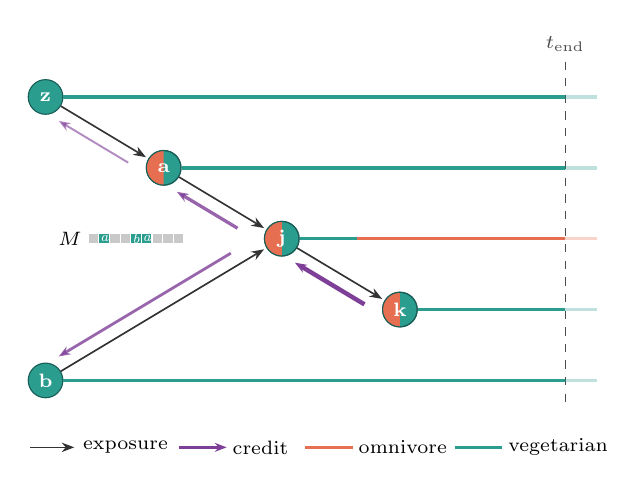
\begin{tikzpicture}[
  x=1cm, y=1cm,
  agent/.style={circle, draw=veg!60!black, fill=veg, minimum size=0.44cm, inner sep=0pt},
  lbl/.style={font=\scriptsize\bfseries, text=white, inner sep=0pt},
  expo/.style={-{Stealth[length=1.6mm]}, black!80, line width=0.6pt, shorten >=1pt},
  cred/.style={-{Stealth[length=1.5mm]}, credit},
  vegline/.style={veg, line width=1.3pt, line cap=butt},
  omnline/.style={omn, line width=1.3pt, line cap=butt},
]

% ---- agents, placed by conversion time (x); z and b start vegetarian ----
\node[agent] (z) at (0,0)      {};
\node[agent] (a) at (1.5,-0.9) {};
\node[agent] (j) at (3.0,-1.8) {};
\node[agent] (k) at (4.5,-2.7) {};
\node[agent] (b) at (0,-3.6)   {};
% converters: omnivore half before, vegetarian half after
\foreach \n in {a, j, k} {
  \begin{scope}
    \clip ($(\n.center)+(-0.3,-0.3)$) rectangle ($(\n.center)+(0,0.3)$);
    \fill[omn] (\n.center) circle (0.22);
  \end{scope}
  \draw[veg!60!black] (\n.center) circle (0.22);
}
\foreach \n in {z, a, j, k, b} { \node[lbl] at (\n) {\n}; }

% ---- analysis window ----
\def\tend{6.6}
\def\tfar{7.0}
\draw[black!70, dashed, line width=0.4pt] (\tend,0.45) -- (\tend,-3.95)
  node[above, pos=0, font=\scriptsize] {$t_{\mathrm{end}}$};

% ---- diet timelines after conversion; j reverts to omnivore ----
\foreach \n in {z, a, k, b} {
  \draw[vegline] (\n.east) -- (\tend, 0 |- \n.center);
  \draw[vegline, opacity=0.3] (\tend, 0 |- \n.center) -- (\tfar, 0 |- \n.center);
}
\draw[vegline] (j.east) -- (3.95,-1.8);
\draw[omnline] (3.95,-1.8) -- (\tend,-1.8);
\draw[omnline, opacity=0.3] (\tend,-1.8) -- (\tfar,-1.8);

% ---- exposure: who was in whose memory buffer at conversion ----
\draw[expo] (z) -- (a);
\draw[expo] (a) -- (j);
\draw[expo] (b) -- (j);
\draw[expo] (j) -- (k);

% ---- j's memory buffer at conversion: 9 samples, a twice, b once ----
\begin{scope}[shift={(0.55,-1.86)}]
  \node[font=\scriptsize, anchor=east, inner sep=1pt] at (-0.05,0.06) {$M$};
  \foreach \i/\s in {0/, 1/a, 2/, 3/, 4/b, 5/a, 6/, 7/, 8/} {
    \ifx\s\empty
      \fill[cell] (\i*0.135, 0) rectangle ++(0.12, 0.12);
    \else
      \fill[veg] (\i*0.135, 0) rectangle ++(0.12, 0.12);
      \node[font=\fontsize{3.5}{4}\selectfont\itshape, text=white, inner sep=0pt]
        at (\i*0.135+0.06, 0.06) {\s};
    \fi
  }
\end{scope}

% ---- credit from k's conversion, walking back through the events, drawn alongside
%      each exposure edge on the side away from the timelines; width = share, fading = depth ----


\draw[cred, line width=1.6pt]
  ($($(k)!0.42cm!(j)$) + (-0.09,-0.15)$) -- ($($(j)!0.30cm!(k)$) + (-0.09,-0.15)$);
\draw[cred, line width=1.2pt, opacity=0.8]
  ($($(j)!0.55cm!(a)$) + (-0.09,-0.15)$) -- ($($(a)!0.30cm!(j)$) + (-0.09,-0.15)$);
\draw[cred, line width=1.0pt, opacity=0.8]
  ($($(j)!0.65cm!(b)$) + (-0.09,0.15)$) -- ($($(b)!0.30cm!(j)$) + (-0.09,0.15)$);
\draw[cred, line width=0.7pt, opacity=0.6]
  ($($(a)!0.42cm!(z)$) + (-0.09,-0.15)$) -- ($($(z)!0.30cm!(a)$) + (-0.09,-0.15)$);

% ---- legend ----
\begin{scope}[shift={(0,-4.45)}, font=\scriptsize]
  \draw[expo] (-0.2,0) -- (0.4,0);   \node[anchor=west, inner sep=2pt] at (0.4,0) {exposure};
  \draw[cred, line width=1.2pt] (1.7,0) -- (2.3,0); \node[anchor=west, inner sep=2pt] at (2.3,0) {credit};
  \draw[omnline] (3.3,0) -- (3.9,0); \node[anchor=west, inner sep=2pt] at (3.9,0) {omnivore};
  \draw[vegline] (5.2,0) -- (5.8,0); \node[anchor=west, inner sep=2pt] at (5.8,0) {vegetarian};
\end{scope}

\end{tikzpicture}
\end{document}
